\documentclass{article}

\usepackage{amsmath, amsthm, amssymb, amsfonts}
\usepackage{thmtools}
\usepackage{graphicx}
\usepackage{setspace}
\usepackage[a4paper, top=0in, bottom=1in, left=.5in, right=.5in]{geometry}
\usepackage{float}
\usepackage{hyperref}
\usepackage[utf8]{inputenc}
\usepackage[latvian]{babel}
\usepackage{framed}
\usepackage{microtype}
\usepackage[dvipsnames]{xcolor}
\usepackage{indentfirst}
\usepackage{tcolorbox}
\usepackage{fontspec}
\usepackage{makeidx}
\usepackage{mathtools}
\usepackage{amsmath}

\DeclareMathSizes{10}{14}{8}{6}
\pagestyle{empty}

\graphicspath{{img/}}
\setmainfont{DejaVu Serif}


\colorlet{LightGray}{White!90!Periwinkle}
\colorlet{LightOrange}{Orange!15}
\colorlet{LightGreen}{Green!15}

\newcommand{\HRule}[1]{\rule{\linewidth}{#1}}

\declaretheoremstyle[name=Theorem,]{thmsty}
\declaretheorem[style=thmsty,numberwithin=section]{theorem}
\tcolorboxenvironment{theorem}{colback=LightGray}

\declaretheoremstyle[name=Proposition,]{prosty}
\declaretheorem[style=prosty,numberlike=theorem]{proposition}
\tcolorboxenvironment{proposition}{colback=LightOrange}

\declaretheoremstyle[name=Principle,]{prcpsty}
\declaretheorem[style=prcpsty,numberlike=theorem]{principle}
\tcolorboxenvironment{principle}{colback=LightGreen}

\setstretch{1.2}
\geometry{
    textheight=9in,
    textwidth=5.5in,
    top=1in,
    headheight=12pt,
    headsep=25pt,
    footskip=30pt
}

\makeindex
% ------------------------------------------------------------------------------

\begin{document}

\section{Kompleksie skaitļi}

\subsection{Algebriskais pieraksts}

Skaitļus $3+2i$, $3-2i$ sauc par kompleksi saistītiem.
\begin{equation}
	(a+bi)(a-bi)=a^2-(bi)^2=a^2+b^2
\end{equation}

Izmantojot šo īpašību, kompleksos skaitļus varam iemācīties dalīt.

\begin{equation}
	\frac{a+bi}{x+yi}
	= \frac{(ax+by)(-ay+bx)i}{x^2+y^2}
\end{equation}

Kvadrāsakni no algebriskā pierakstā rakstītiem kompleksiem skaitļiem var vilkt ar formulu:
\begin{equation}
	\sqrt{a+bi}=\pm
	\left(
	\sqrt{\frac{\sqrt{a^2+b^2}+a}{2}+\beta i\sqrt{\frac{\sqrt{a^2+b^2}-a}{2}}}
	\right)
\end{equation}

Kompleksos skaitļus algebriskā pierakstā varam attēlot kompleksajā planknē.

\begin{center}
	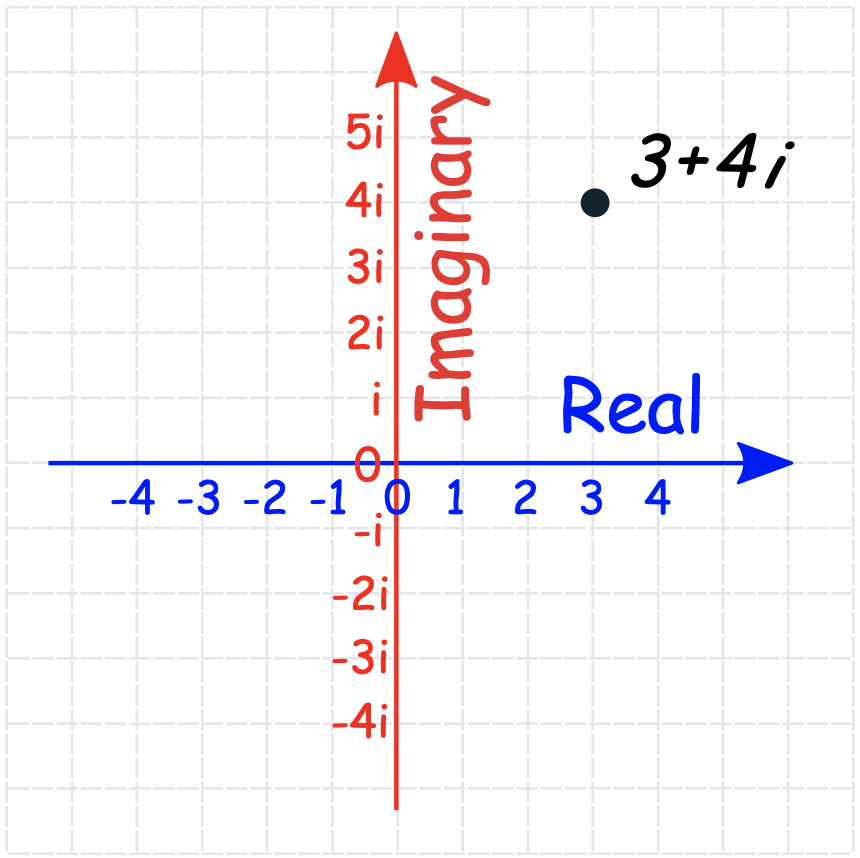
\includegraphics[width=.4\linewidth]{complex_plane-1}
\end{center}

\subsection{Trigonometriskais pieraksts}

Kompleksu skaitli $z =a+bi$ kā plaknes punktu var uzdot arī ar: polāro rādiusu $r$ (skaitļa moduli, jeb absolūto vērtību, $r=|z|$) un polāro leņķi $\varphi$ (skaitļa argumentu, $\varphi=arg(z)$).

Moduļa aprēkināšana:
\begin{equation}
	r=\sqrt{a^2+b^2}
\end{equation}

Reizinot divus kompleksus skaitļus, trigonometriskajā pierakstā
viss sanāk ļoti vienkārši un simetriski:
\begin{equation}
	zz'=rr'(\cos(\varphi+\varphi')+i\sin(\varphi+\varphi'))
\end{equation}

\textbf{Teorēma.} Komplekso skaitļu reizinājuma modulis ir reizinātāju moduļu reizinājums, bet reizinājuma arguments – reizinātāju argumentu summa.

Pieņemsim, ka skaitlis z' nav 0. Tad:
\begin{equation}
	\frac{z}{z'}=\frac{r}{r'}(\cos(\varphi-\varphi')+i\cos(\varphi-\varphi'))
\end{equation}

Kāpināšana:
Ja $n>1$, tad $z^n$ apzīmē $z\cdot\ldots\cdot z$ (n reizes).

Teorēma: Ja $m,n>1$, tad:

\begin{align}
	&z^m z^n = z^{m+n}; \\
	&(z^m)^n=z^{mn}
\end{align}

\section{Polinomi}


Polinoms - [TK def]

\subsection{Teorēmas}
Quotient-Remainder

\subsection{Lielākais kopīgais dalītājs}
Definīcijas

\subsection{Polinoma būvēšana}
\subsubsection{Dabiskā metode}
\subsubsection{TK Matrica (vispārīgi)}

\section{Gredzeni un Lauki}

\end{document}